\chapter{优化中微子望远镜设计}
\label{chap:telescope_design}

\section{使用hDOM来提升角分辨率}
\label{sec:hdom}

海铃中微子望远镜的一大特点是使用了全新的hDOM\cite{hDOM:2021}来作为其探测切伦科夫光的模块,它即包含传统的PMT,又包含新型的光敏元件——SiPM(silicon photon multiplier)。

\subsection{SiPM的特点}

SiPM是一种硅基的光敏探测元件,它是由成百上千个处于盖革工作状态下的雪崩光电二极管(photon avalanche diodes,PAD)所铺设构成的\cite{understanding_sipm:2019}。由于这些PAD处于盖革工作状态,即当有一个光子到达其表面,激发出电子空穴对时,便能在外部电场的作用下形成雪崩效应,因此它们也被称为SPAD(single photon avalanche diodes)。
相比于传统的PMT,SiPM具有许多独特的优点:
\begin{enumerate}
    \item SiPM中的SPAD内部的尺寸结构很小,其内部的雪崩发展及其迅速而稳定,因此SiPM拥有极佳的时间响应性能,理论上可以达到$\sim 10\,\mathrm{ps}$。而PMT中光子需要经过多个倍增极的放大,因此有$10 ~ 20\,\mathrm{ns}$的渡越时间(transient time,TT),而渡越时间弥散(transient time spread,TTS)通常在$1~5\,\mathrm{ns}$量级。
    \item SiPM中的SPAD通过光子激发电子空穴对的量子效率可以达到$\gtrsim 50 \%$,而PMT中借助光子激发出能够离开阴极材料的自由电子的量子效率仅为$\sim 30\%$。
    \item SiPM中的SPAD对单光子响应产生的电流大小非常稳定,因而具有很好的单光子分辨能力。
    \item SiPM中的PAD只需要加上几个伏特的偏置电压即可处于盖革工作模式,达到预设的量子效率和增益效果。而PMT则需要加上$\gtrsim 1000 \,\mathrm{V}$的高压才能达到稳定的增益,因而需要在探测器内部添加额外的升压电路模块,。
    \item 作为一种硅基的固态探测器,SiPM是的仪器体积小集成程度高,可以搭载在各种不同的探测设备上。而PMT是一个真空玻璃管,更容易受到损坏,日本的神冈探测器就曾经因为PMT真空管爆炸引发连锁反应,直接毁掉了近半个探测器的PMT。为防止类似事件的发生,JUNO中的PMT外部均额外安装了保护壳\cite{JUNO_pmt_implosion:2022}。
    \item 在批量生产下,SiPM作为一种硅基晶体材料,可以在流水线的形式快速地加工出来,因而可以有效降低成本。而PMT的制造过程中依赖于许多人力帮助,批量生产的效率并不高。
\end{enumerate}

当然,SiPM也有其自身的缺点,其最大的问题便是在室温下噪声非常地高。SiPM中由于晶体自身的结构缺陷,很容易通过热涨落的形式产生暗噪声,常见的型号在室温下噪声率在$100\,\mathrm{kHz/cm^2}$的量级。
此外SiPM内部的串扰也相对较大,一个雪崩的SPAD可能会激发与之相邻的SPAD,从而对一个单光子事件产生多光子的响应信号。

由于这些特点,SiPM目前已经在雷达激光测距(LIDAR)\cite{sipm_lidar:2013},医学造影\cite{nuclear_medical_imaging:2009},JUNO-TAO探测器\cite{JUNO-TAO:2023},对撞机的闪烁体探测器\cite{SiPM_CEPC:2020}等多个领域都有所应用。
在本节后续的内容中,我们将讨论SiPM在中微子望远镜中的潜在应用。

\subsection{hDOM性能分析}

在本研究中,我们主要考虑SiPM的快速时间响应能力和高量子效率对中微子望远镜中的径迹方向重建精度的提升。
我们以KM3NeT的mDOM设计为基础结构\cite{KM3NeT_mDOM:2015},在其中额外加入了24个SiPM阵列,每一个SiPM阵列由$9 \times 9$个SiPM单点构成,有$2.7\times 2.7\,\mathrm{cm}$的面积,它们组成了4个水平的环带,插入在PMT中间。
我们将24个SiPM和31个PMT同时加入到数字光学模块中,构成了一个混合数字光学模块(hDOM),其初步设计图如图\ref{fig:hDOM_rendering}中所示。

为了研究量子效率和时间分辨率对探测器性能的影响,我们在模拟中假设了三种不同的光敏探测器,其参数列表分别如表格\ref{tab:sensor_parameters}中所示。

\begin{table} [htbp]
    \centering
    \begin{tabular}{c|c|c|c}
        \hline
        光敏元件 & PMT & toy SiPM & SiPM  \\
        \hline
        物理体积 [$\rm{cm}^2$] & 40.7  & 40.7 & 7.3 \\
        \hline
        $405\,\mathrm{nm}$下光子探测效率 [\%] & 24 & 24 & 42 \\
        \hline
        时间分辨率 [$\rm{ns}$] & 5 & 0.1 & 0.1 \\
        \hline
    \end{tabular}
    \caption{三种不同的探测元件的性能参数}
    \label{tab:sensor_parameters}
\end{table}

使用这些不同的光敏元件,我们可以组件如下所示的三种不同的光学模块的配置:
\begin{enumerate}
    \item 配置A,由31个PMT构成的光学模块,即形如KM3NeT的mDOM。
    \item 配置B,由31个物理面积和量子效率与PMT相同,但是拥有极佳时间分辨性能的toy SiPM(或者也可以称为是高时间分辨率的PMT)构成的光学模块。
    \item 配置C,由31个PMT和24个标准的SiPM所构成的混合光学模块,即我们的hDOM。
\end{enumerate}
其中,我们的hDOM拥有适中的时间分辨率和最大的光敏面积。利用章节\ref{subsec:hDOM_sim}介绍过的模拟程序,我们模拟了hDOM对来自不同方向的平行光的响应,其内部各个光敏元件所对应的有效光子接收面积如图\ref{fig:hdom_effective_area}中所示。

\begin{figure}[!htb]%
    \centering
    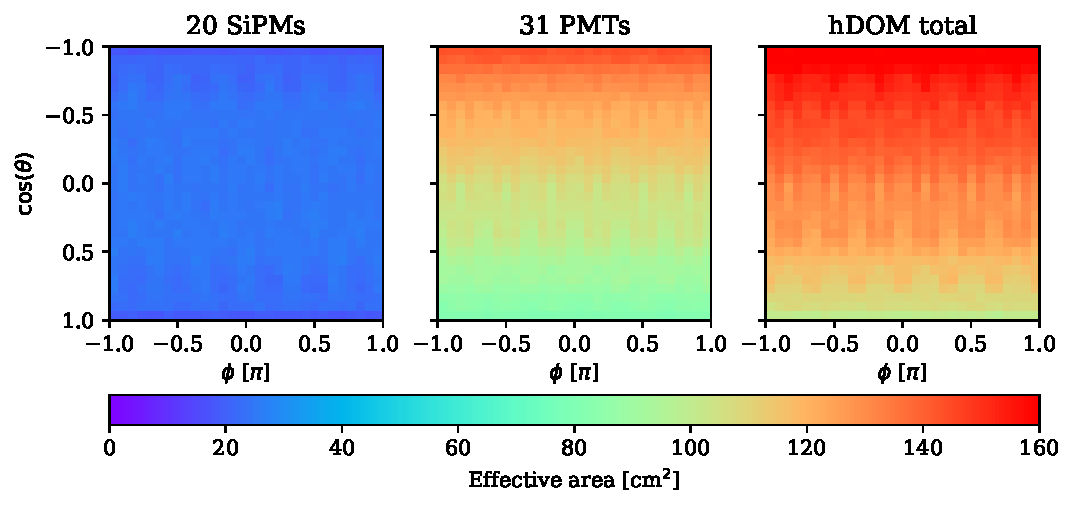
\includegraphics[width=0.90\textwidth]{img/hdom_effective_area.pdf}
    \caption{hDOM中各个光敏元件组分的有效光子接收面积随光子入射角的关系。}
    \label{fig:hdom_effective_area}
\end{figure}

在完成对光敏元件的假设和构建完光学模块之后,我们研究的主要内容便是探讨不同的光敏模块对径迹型事件的响应,其中我们着重关心在不同光敏模块配置下阵列对缪子径迹的角度分辨率。

为提高模拟的效率,我们配置了一个相对紧凑的$1\,\mathrm{km^3}$体积的阵列,它在$x$,$y$和$z$方向上分别均匀得分布着$10 \times 10 \times 50$个光学模块,总共包含了5000个光学模块。
我们将介质的光学性质分别设置成深海海水和南极冰川冰,其中南极冰川比相对于深海海水具有更长的吸收长度和更短的散射长度\cite{OP_IceCube:2013, OP_KM3NeT_LAMS:2011}。对着两种介质,我们分别进行了模拟,从而比较不同配置的光学模块在不同介质下的表现。

我们在探测器阵列中注入了大批量的$1\,\mathrm{TeV}$的缪子径迹型数据,在模拟得到切伦科夫光子打在光学模块表面的光子击中信息后,我们利用我们设计的hDOM模拟程序分别模拟不同光学模块配置下,光敏元件对入射光子的响应。
随后我们根据表\ref{tab:sensor_parameters}中的配置来模拟光敏元件对光子的探测效率和时间测量精度,并最终用章节\ref{sec:angular_resolution}中介绍的径迹重建算法来对径迹型事件进行重建,根据重建结果得到阵列的角分辨率。

我们的模拟和重建结果显示,对于$1\,\mathrm{TeV}$的缪子径迹型事件而言,不同配置下的探测器对缪子信号的重建精度如图\ref{fig:hdom_angular_resolution_total}中所示。
我们发现在海水中相比于普通的mDOM(配置A),hDOM(配置C)能够带来$\sim40\%$的角度分辨率提升。而通过对比普通的mDOM(配置A)和由toy SiPM构成的DOM(配置B),我们可以发现,光敏元件的时间分辨率对角度重建性能有至关重要的影响。
与此同时,在冰介质中,hDOM(配置C)和由toy SiPM构成的DOM(配置B)相比于普通的mDOM(配置A)的提升并不明显,仅为$\sim 10\%$的量级。这是由于冰介质中的散射效应明显,因此光子到达时间的测量实际上是由散射效应所主导的,而非光敏元件自身的时间分辨率。

我们的研究表明SiPM的高时间精度和高量子效率的特点可以极大地提高中微子望远镜阵列的角度分辨率。
但是在真实的中微子望远镜阵列中,还有一些其他因素会影响hDOM的时间精度:
阵列的时钟同步性能,目前我们计划使用的小白兔系统\cite{white_rabbit:2013}大约能提供$< 100 \,\mathrm{ps}$的时钟同步精度;
hDOM的定位精度,KM3NeT的声学定位系统\cite{KM3NeT_acoustic:2022}可以达到$\sim 10 \,\mathrm{cm}$的定位精度,对应$\sim 400 \mathrm{ps}$的光子传播时间;
由海水色散关系导致的切伦科夫光的到达时间弥散等等。
对于这些实验中需要考虑的情形,我们还需要更多的研究才能准确地确定hDOM的性能优势。


\begin{figure}[!htb]%
    \centering
    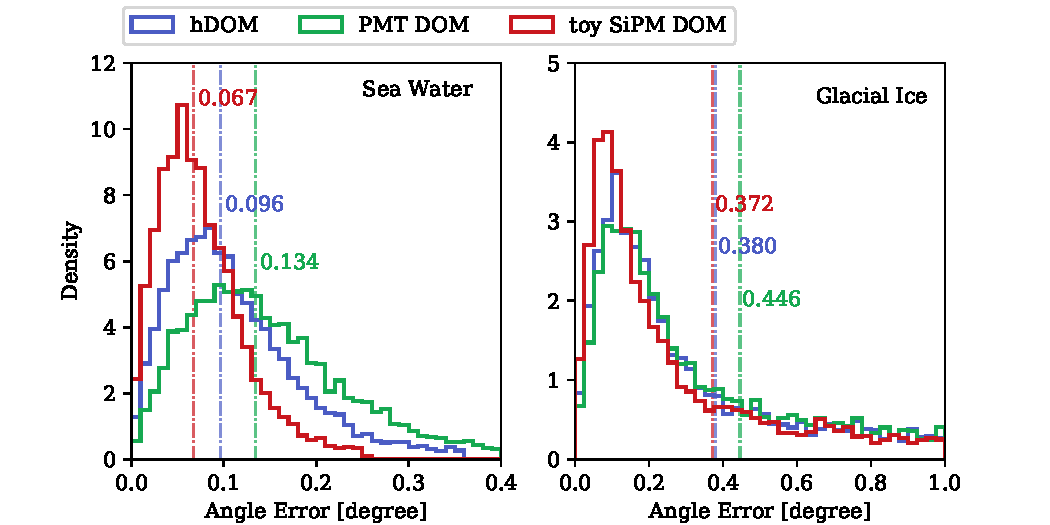
\includegraphics[width=0.95\textwidth]{img/hdom_angular_resolution_total.pdf}
    \caption{不同配置下的光学模块对$1\,\mathrm{TeV}$的缪子径迹型事件的重建角分辨率。左图为在深海海水中的情况,而右图对应在南极冰川冰中的情况。}
    \label{fig:hdom_angular_resolution_total}
\end{figure}





\section{彭罗斯构型来作为串列单元的排布}

\subsection{彭罗斯构型介绍}

海铃中微子望远镜的串列单元的几何布局设计中采用了彭罗斯构型,在不考虑机器人过道后,阵列的布局如图\ref{fig:geo_layout_penrose}所示。
在彭罗斯构型中,串列单位的位置对应于彭罗斯镶嵌中的多边形的顶点位置,而彭罗斯镶嵌是一种非周期性密铺\cite{tilings_and_patterns:1987},其形状如图\ref{fig:Penrose_tiling_wiki}中所示。
彭罗斯镶嵌的最大特点是它不具备平移周期性,因此从宏观上看,空间中的每一个点都与其他的点周围的结构互不相同的。
尽管如此,彭罗斯镶嵌具有10个镜面对称轴和5重旋转对称性。

彭罗斯镶嵌的几何结构参考了黄金三角形中的一些规律,它可以由两种基本黄金三角形逐渐细分演变而来,其细分的过程如图\ref{fig:penrose_iteration}。因此,彭罗斯镶嵌还具有一些分形几何结构的特点:图案具有自相似性,而且在几次细分之后图案中存在一些相同的微小结构。

\begin{figure}[!htb]%
    \centering
    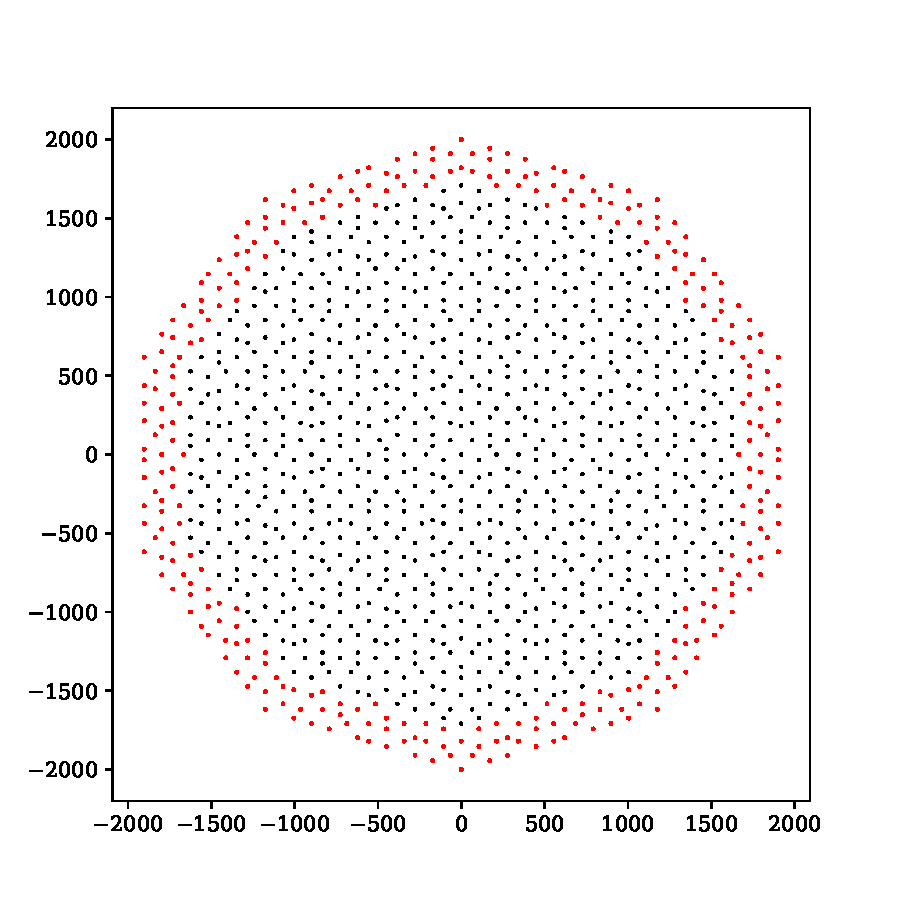
\includegraphics[width=0.80\textwidth]{img/geo_layout_penrose.pdf}
    \caption{彭罗斯构型下,串列单元在水平方向上的排布。每一个点表示一根串列单元,其中红色加粗的点表示在外围用于屏蔽的串列单元。}
    \label{fig:geo_layout_penrose}
\end{figure}

\begin{figure}[!htb]%
    \centering
    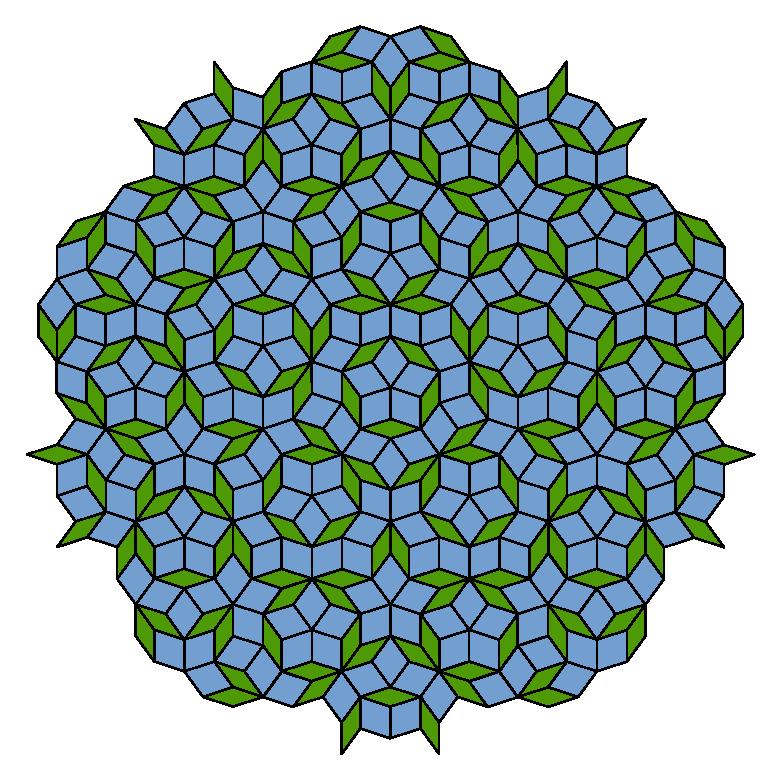
\includegraphics[width=0.70\textwidth]{img/Penrose_tiling_wiki.pdf}
    \caption{彭罗斯镶嵌的示意图,图片来自于维基百科。}
    \label{fig:Penrose_tiling_wiki}
\end{figure}

\begin{figure}[!htb]%
    \centering
    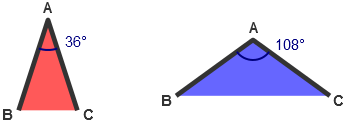
\includegraphics[width=0.55\textwidth]{img/penrose_triangles.png}
    \vskip 1cm
    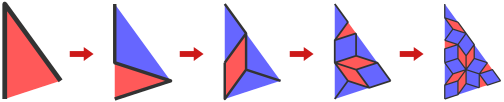
\includegraphics[width=0.75\textwidth]{img/penrose_splite.png}
    \vskip 1cm
    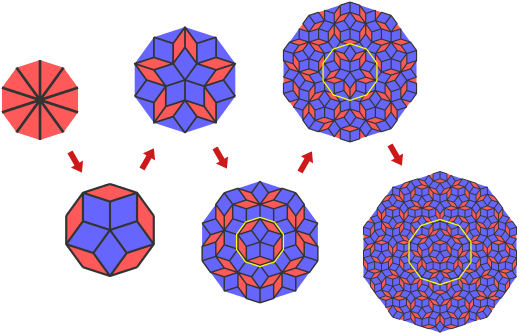
\includegraphics[width=0.90\textwidth]{img/penrose_iteration.png}
    \caption{通过迭代细分黄金三角形的方式得到彭罗斯镶嵌的过程。}
    \label{fig:penrose_iteration}
\end{figure}


\subsection{主要优点}

将彭罗斯构型应用于中微子望远镜之中,有两个主要的优点,一是阵列中的串列单元密度分布具有疏密相间的特点,从而提高对簇射型事件的灵敏能量范围,二是阵列中没有明显的方向性,可以避免径迹型事件沿着某个特定地方向偷偷溜过而没有留下信号。

对于第一个优点,我们可以发现彭罗斯构型中的串列单元之间并非是等间距的。如果统计每一根串列单元距离与之最近的5根串列单元的距离,我们可以得到串列单元之间的水平间距分布如图\ref{fig:distance_spectrum_penrose}中所示。
我们可以发现构型中有两个典型的距离,分别是$68.9\,\mathrm{m}$和$111.5\,\mathrm{m}$,分别对应图\ref{fig:Penrose_tiling_wiki}中绿色四边形的相近的两个对立顶点的距离和边长,这两个距离构成了黄金分割比$G = (\sqrt{5}+1)/2$。

\begin{figure}[!htb]%
    \centering
    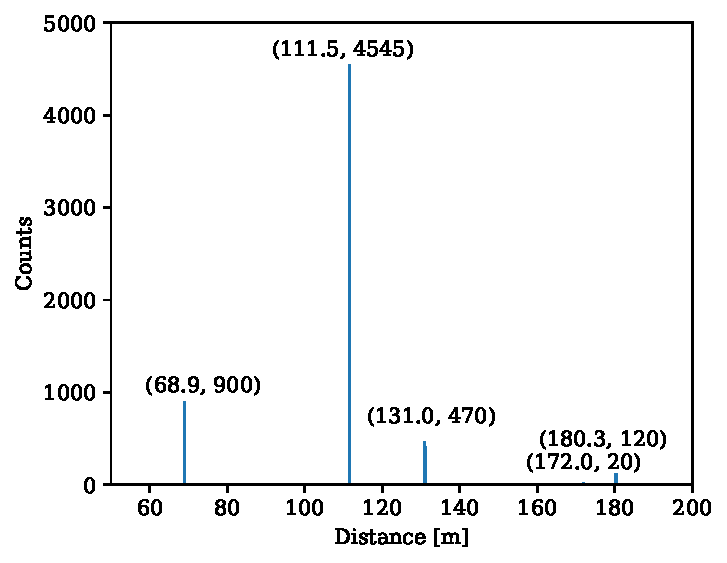
\includegraphics[width=0.65\textwidth]{img/distance_spectrum_penrose.pdf}
    \caption{彭罗斯构型中串列单元之间的水平间距分布图。}
    \label{fig:distance_spectrum_penrose}
\end{figure}

要更为细致地讨论几何构型中串列单元在空间上的密度分布,需要指定一个观察区域大小,该观察区域的大小设置将会对密度分布的均匀性有重要的影响。
如果观察区域设置得过小,例如远小于串列单元之间的间距,则我们将会观察到由单个串列单元引起的不均匀性。反过来,如果观察区域设置得远远大于串列单元之间的间距,则密度不均匀性将会被抹平。
在我们的分析中,我们以中微子望远镜的观察对象——中微子事件来作为参照系。
对于径迹型事件而言,它是一条很长的能够横穿探测器的径迹,因此在径迹型事件中探测器的几何分布始终是相对均匀的。
对于簇射型事件,粒子簇射的发展尺度约为$10\,\mathrm{m}$,而水的吸收长度约为$25\,\mathrm{m}$,因此簇射型事件的信号是相对局域的。对于某一个簇射型事件,只有它周围一小部分的串列单元能够观察到它的信号。
对簇射型事件的模拟表面,半径在$100\,\mathrm{m}$内的串列有较大概率接收到信号,因此我们选择以一个半径为$100\,\mathrm{m}$的圆来作为观察区域。

在实际操作中,我们将图\ref{fig:geo_layout_penrose}中所示的阵列的位置与一个$sigma = 100\,\mathrm{m}$的二维高斯函数做卷积,其结果如图\ref{fig:string_density_penrose}中所示。
从图中我们可以观察到,彭罗斯构型中分布着一些大小约$50\,\mathrm{m}$的高密度区域和大小约$100\,\mathrm{m}$的低密度区域。
相比于发生在低密度区域中的簇射型事件,发生在高密度区域中的簇射型事件能够被多$\sim30\%$的临近串列所观察到,从而接收到更多的光子信息,这意味着高密度区域的阵列对簇射型事件的能量阈值会有所降低。

\begin{figure}[!htb]%
    \centering
    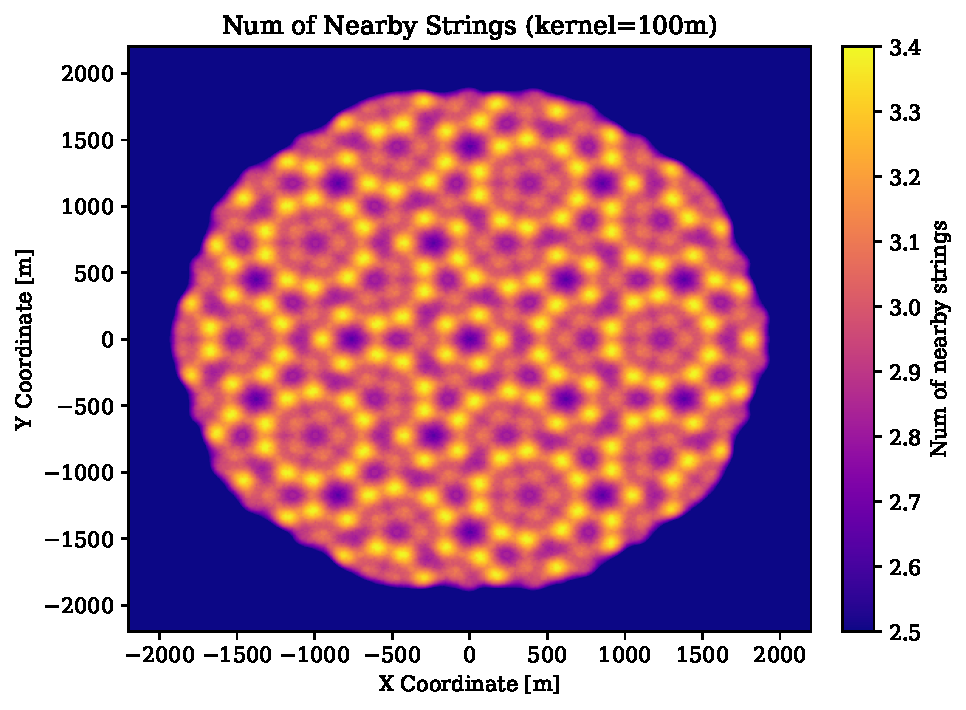
\includegraphics[width=0.85\textwidth]{img/string_density_penrose.pdf}
    \caption{在观测的分辨率为一个$sigma = 100\,\mathrm{m}$的二维高斯函数的情况下,观测到的彭罗斯构型的串列单元的密度分布。}
    \label{fig:string_density_penrose}
\end{figure}

这种高密度区域和低密度区域混合的几何排布能够用高密度区域观测更低能量的簇射型事件,而低密度区域则负责以较低的成本扩大阵列的监控体积,从而扩宽探测器的灵敏能量范围。
有关不同几何构型下对簇射型事件的灵敏度能量范围的定量影响,将在未来簇射型事件的分析流程更加完备后发布。

彭罗斯几何构性的第二个优点将会提高我们对筛选发生在探测器内部的中微子事件的筛选效果。
来自探测器顶部上方的中微子源发射的中微子信号是向下穿行至探测器的,而中微子望远镜探测到的向下穿行的事件中含有很强烈的大气缪子噪声。
通常,人们会选用顶点发生在探测器内的事件来屏蔽大气缪子噪声,这是因为大气缪子是产生在大气层中的,他们在到达探测器的过程中必然会由探测器的边缘进入。
通过屏蔽到在事件开始的一段时间内(例如$500\,\mathrm{ns}$)有在阵列边缘的串列单元中留下信号的事件,我们便可以挑选出来自DIS过程发生探测器内部的中微子事件\cite{IceCube_HESE:2020}。
这种筛选方法在屏蔽大气缪子事件的同时,也能屏蔽一部分的大气中微子事件\cite{IceCube_starting_track:2021},这是因为大气中微子是大气缪子一同产生的。

此时阵列边缘的那一部分串列单元的屏蔽效率对于分析而言便起着至关重要的作用。
在本次分析中,我们选取外侧320根串列单元来作为屏蔽层,其位置如图\ref{fig:geo_layout_penrose}中的红点所示。

我们研究当一根$1\,\mathrm{TeV}$的缪子径迹距离串列单元多近的时候,能够被串列单元上面的hDOM探测到。
对于缪子径迹型事件而言,它发射的切伦科夫光朝着切伦科夫角方向运动。对于到径迹距离为$d$的探测器而言,它探测到的光子数$N_\mathrm{obs} (d)$为:
\begin{equation}
    N_\mathrm{obs} (d) = 
    \frac{\mathrm{d}N}{\mathrm{d}x}
    \frac{1}{2 \pi d} e^{-d/(\cos\theta_\mathrm{CK} \,\lambda_\mathrm{abs})} 
    \times A_\mathrm{obs} ,
\end{equation}
其中$\frac{\mathrm{d}N}{\mathrm{d}x} \simeq 1500 \,\mathrm{photons/cm}$是$1\,\mathrm{TeV}$的缪子在水中的平均光产额,$\lambda_\mathrm{abs} \simeq 25\,\mathrm{m}$为海水的吸收长度,$\theta_\mathrm{CK} = 0.74$表示切伦科夫角,$A_\mathrm{obs} \simeq 120\,\mathrm{cm^2}$表示hDOM中PMT对方向光的有效面积。
要求$N_\mathrm{obs} (d_c) = 1$,我们得到临界距离$d_c \simeq 35\,\mathrm{m}$。
值得注意的是临界距离选择与考察的缪子的能量有关,对于更加低能的事件,其对应的临界距离也会更短一些。

对于来自某个方向的$1\,\mathrm{TeV}$的缪子,我们把每一个外围屏蔽层中的串列单元都用一个$\sigma = 35\,\mathrm{m}$的二维高斯函数来做卷积,我们观察缪子穿行路径上串列单元密度的积分,由此来表示缪子经过的串列单元的数量。
对于沿着$x$轴正向运动的缪子,它穿越的串列单元的数量与缪子径迹与坐标系原点的截距之间的关系如图\ref{fig:corridor_penrose}中所示。
我们可以看到除了极少数窗口外,绝大多数的缪子穿越的串列单元数量都大于1,即均能被屏蔽层所屏蔽。

\begin{figure}[!htb]%
    \centering
    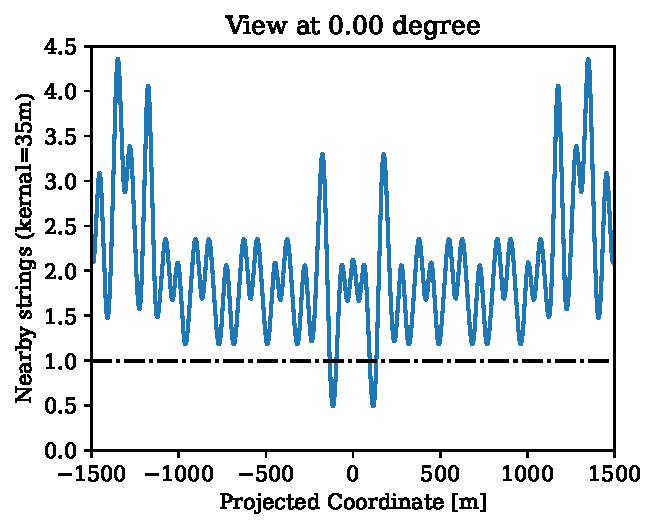
\includegraphics[width=0.60\textwidth]{img/corridor_penrose.pdf}
    \caption{假设每一根外围屏蔽层中的串列单元的影响范围为一个$\sigma = 35\,\mathrm{m}$的二维高斯函数,$1\,\mathrm{TeV}$缪子径迹型事件所穿过的串列单元数量与径迹和坐标原点之间截距的关系图。}
    \label{fig:corridor_penrose}
\end{figure}

我们研究漏过的缪子的截距范围与总截距范围的比值,即缪子事件对屏蔽层的逃逸率,随着入射角度的关系,其结果如图\ref{fig:corridor_angle_penrose}所示。
我们可以看到彭罗斯构型中存在5个相对的缺陷方向,来自那些方向的缪子的逃逸率较高,但是缺陷的程度并不明显,与各个方向的平均值相差较小。

\begin{figure}[!htb]%
    \centering
    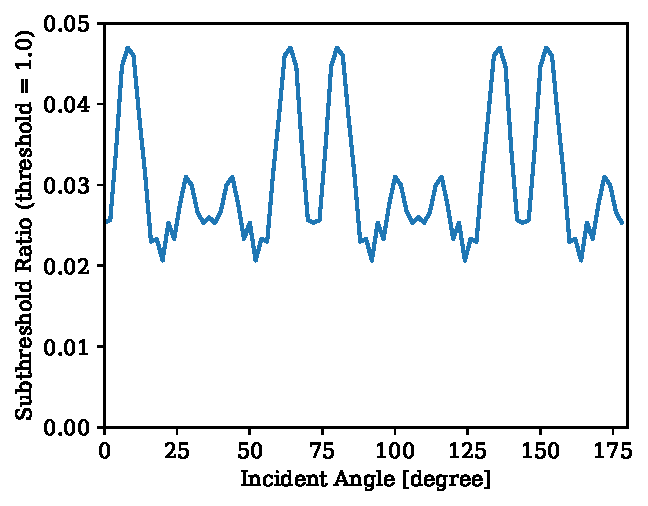
\includegraphics[width=0.60\textwidth]{img/corridor_angle_penrose.pdf}
    \caption{彭罗斯构型下,缪子事件对屏蔽层的逃逸率与缪子入射角度的关系图。}
    \label{fig:corridor_angle_penrose}
\end{figure}

\subsection{与其他构型的对比}

在本小节中,我们将上一小节中对彭罗斯构型的性能分析同样地运用在另外两个典型的构型中,它们分别是向日葵构型和正方形构型。
在对比中,我们控制不同几何构型之间的串列单元的总数和总体的面密度保持不变,均为1211根和$9710\,\mathrm{m^2}$平方米每根。

向日葵构型中串列单元的位置在极坐标系下的表示为:
\begin{equation}
\begin{aligned}
    r_i &= R_0 \sqrt{i} \\
    \phi_i &= \frac{2\pi}{G^2} i ,
\end{aligned}
\end{equation}
其中$i$表示第i根串列单元,从1取到1211,$R_0 = 56\,\mathrm{m}$为阵列的大小因子,$G$是黄金分割比。
向日葵构型下阵列的水平分布如图\ref{fig:geo_layout_sunflower}中所示。
向日葵构型也具有在空间中不对称且不存在特定的方向性的特点,这种构型在IceCube-Gen2\cite{IceCube-Gen2_white_paper:2020}和射电相干阵列\cite{vigano_sunflower:2009}中均有一定的应用研究。
而正方形构型即将阵列以正方形的形式向外扩展,其阵列的水平分布如图\ref{fig:geo_layout_cube}中所示。

向日葵构型和正方形构型都有非常均匀的串列单元的面密度分布,关于向日葵构型中的串列单元水平间距分布和串列单元的密度分布可以参考图\ref{fig:distance_spectrum_sunflower}和图\ref{fig:string_density_sunflower}。
因此它们对阵列中各个位置发生的簇射型时间的响应比较均匀。

向日葵构型在不同的方向观察下也具有非常好的均匀性,它自身没有任何对称轴,在各个方向看来都像是一个均匀的圆盘状,$1\,\mathrm{TeV}$的缪子径迹型事件能够逃逸探测器屏蔽层检测的几率如图\ref{fig:corridor_angle_sunflower}所示。
而正方形构型中存在两个明显的方向,即$x$轴$y$轴方向,沿着这两个方向来的缪子事件有很大的几率直接到达探测器内部而不被外圈的屏蔽层检测到,其逃逸率如图\ref{fig:corridor_angle_cube}中所示。

\section{阵列几何间距对灵敏度的影响}

中微子望远镜中hDOM阵列在空间中的分布间距会对望远镜的灵敏度有重要的影响\cite{IceCube-Gen2_sensitivity:2021, KM3NeT_spacing:2013}。
在串列单元数量和hDOM的总数不变的情况下,hDOM的分布越密集,探测器能够接收到的光子数越多,探测器的的能量阈值越低。
反过来的话,分布越稀疏,探测器的能量阈值越高,但是同时探测器能够监控的海水体积也变多了,因此对高能事件的有效面积会响应地增加。
在本节中,我们通过改变hDOM水平和垂直间距的方式,研究海铃对能谱指数为-3和-2的源的各自的显著性变化。

\subsection{几何参数设置}

在模拟中,我们以章节\ref{sec:TRIDENT_array}中描述的彭罗斯构型为基准设计,在其基础上对hDOM之间的水平和垂直间距进行一定的比例缩放。
在本节中我们研究的缩放因子如图\ref{fig:spacing_scale}中所示。

\begin{figure}[!htb]%
    \centering
    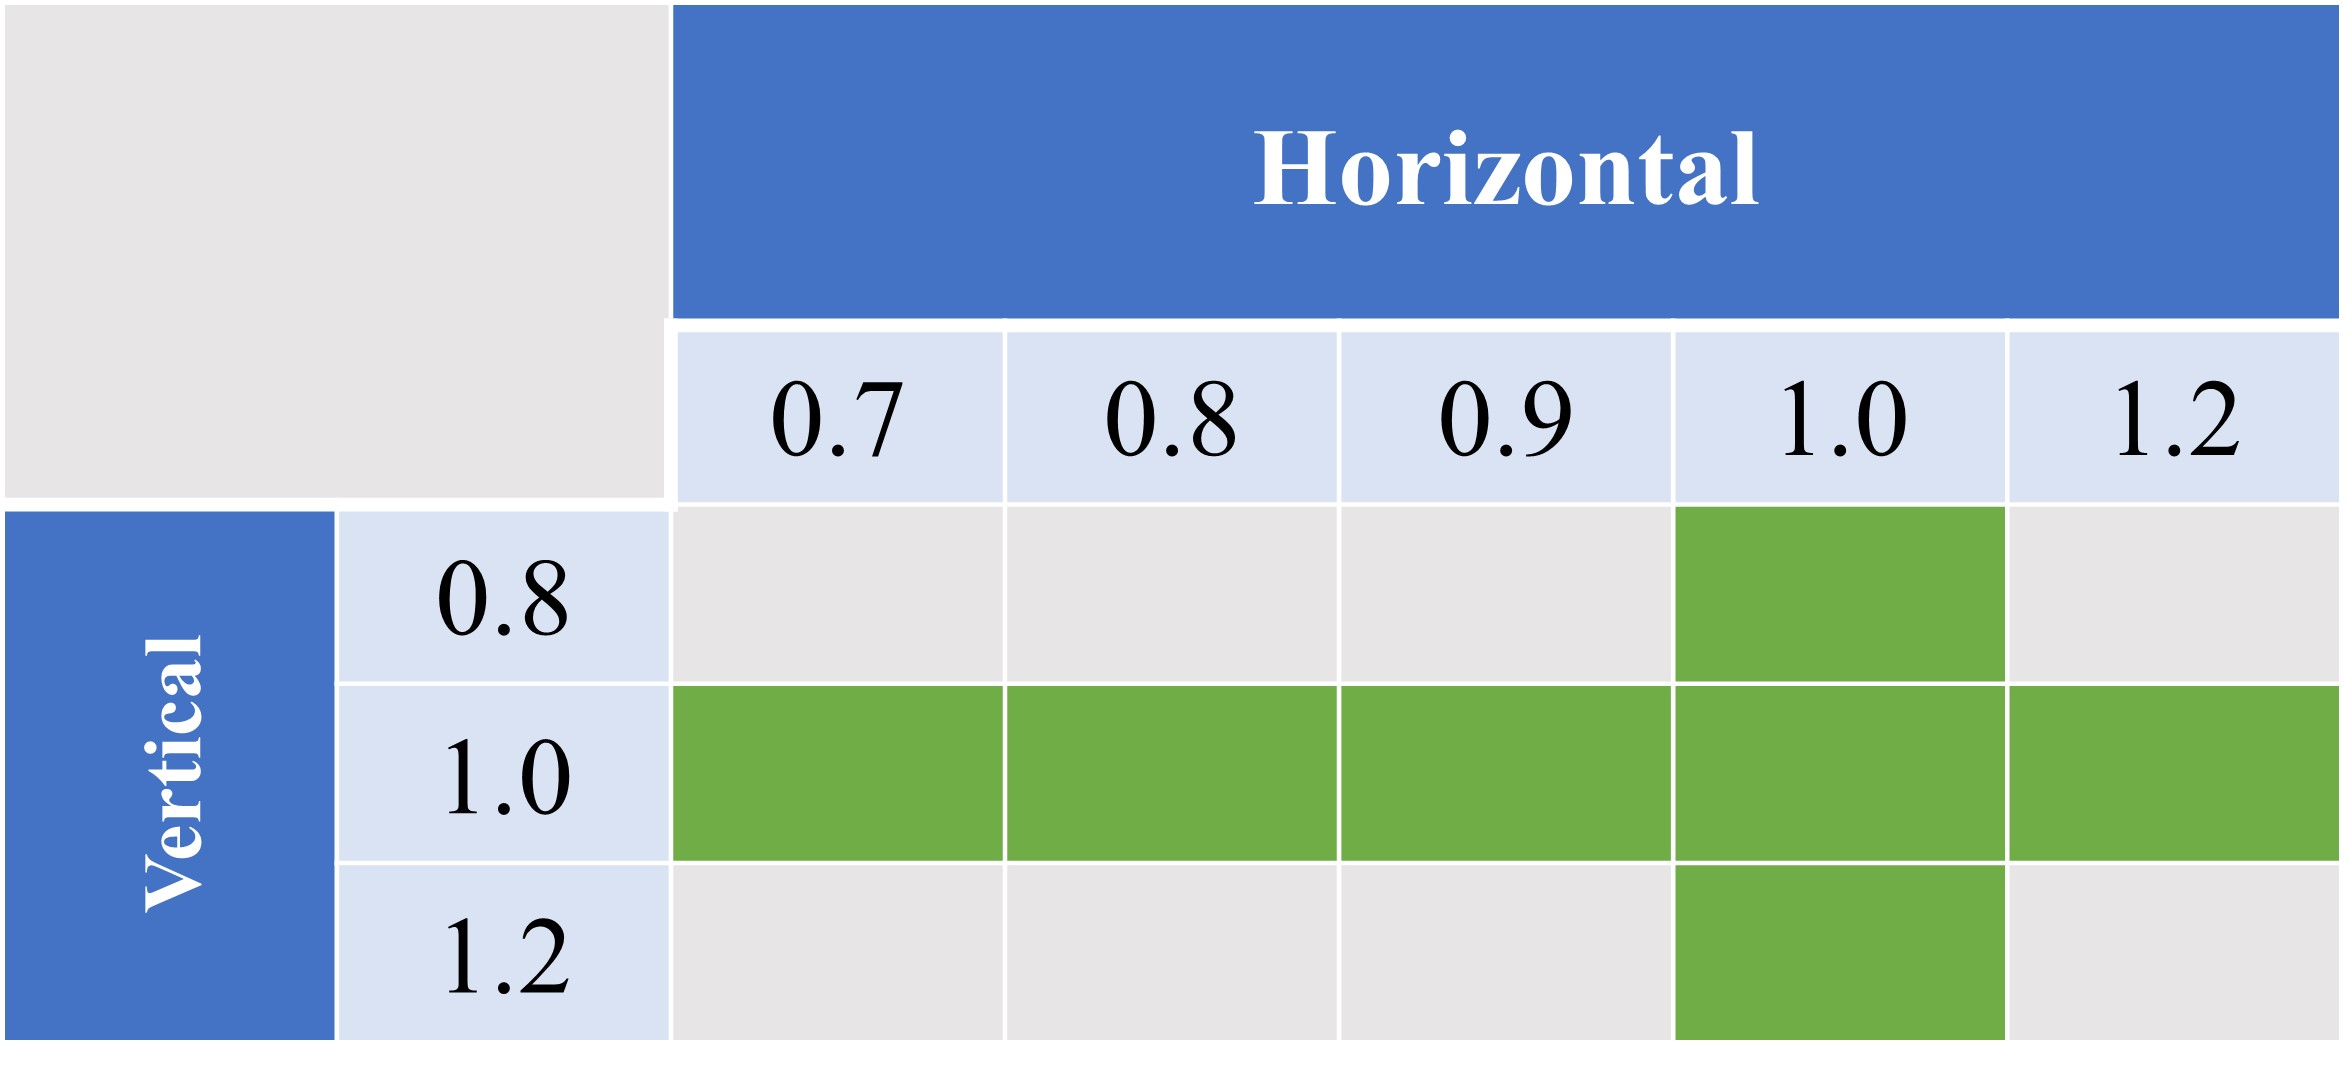
\includegraphics[width=0.70\textwidth]{img/spacing/spacing_scale.jpg}
    \caption{模拟研究中采用的hDOM水平和垂直间距的缩放因子配置图。其中绿色部分为我们进行了模拟和分析的配置。}
    \label{fig:spacing_scale}
\end{figure}

\subsection{对阵列性能影响分析的结果}

对不同配置下的望远镜整列,我们进行了章节\ref{chap:simulation_framework}和\ref{chap:telescope_performance}中所介绍的全面模拟和分析流程,我们的分析对比结果如下所示。


海铃对缪子径迹型事件的角分辨率随着几何间距的变化如图\ref{fig:spacing_angular_resuolution}中所示。我们可以发现在$1\,\mathrm{TeV} - 1\,\mathrm{PeV}$的能量范围内,阵列的水平间距越小,垂直间距越大,中微子望远镜的角分辨率越好。对于能量小于约$10\,\mathrm{TeV}$的事件而言,缩小阵列的垂直间距对角分辨率的影响并不大。

而海铃对来自水平和向上穿行方向的缪子径迹型事件的有效面积变化如图\ref{fig:spacing_effective_area_horizontal}和\ref{fig:spacing_effective_area_up-going}中所示。
我们发现对于水平方向的事件来说,放大水平和垂直间距均能取得比较好的有效面积提升。
而对于向上穿行的事件来说,在放大水平间距会导致其在低能段的有效面积的下降而在高能段上升,而垂直间距的影响非常小。这是由于对于低能的向上飞行的缪子径迹型事件,过大的有效面积可能会导致其能够点亮的hDOM数量过少,从而难以触发探测器。

最终我们研究不同间距下的海铃阵列对中微子望远镜源的灵敏度,对于能谱指数为-2和-3的源,不同间距下的海铃阵列在10年的观测时间内达到$5\sigma$置信度的观测所需的流量对比分别如图\ref{fig:spacing_source_sensitivity_2}和图\ref{fig:spacing_source_sensitivity_3}中所示。
我们发现改变水平间距对赤纬范围为$(-0.6, 0)$范围内的源和其他赤纬范围内的源的影响不同,这是由于这两个赤纬范围内,探测器的曝光时间中来自水平方向的事件的占比不同,正如图\ref{fig:source_zenith_duty_cycle}红线所展示的那样。
而此前关于有效面积的讨论中,我们已经发现了水平间距的变化对于向上穿行和水平方向的径迹型事件的有效面积有不同的影响。

我们对阵列几何间距的研究表明:对于能谱指数为-2的源而言,将水平和垂直间距放大到原先的1.2倍可以有效提高望远镜对该类型的源的灵敏度;而对于能谱指数为-3的源而言,目前的几何间距已经处于一个比较优良的位置,将垂直间距放大到1.2倍可以略微提高望远镜的灵敏度。

\begin{figure}[!htb]%
    \centering
    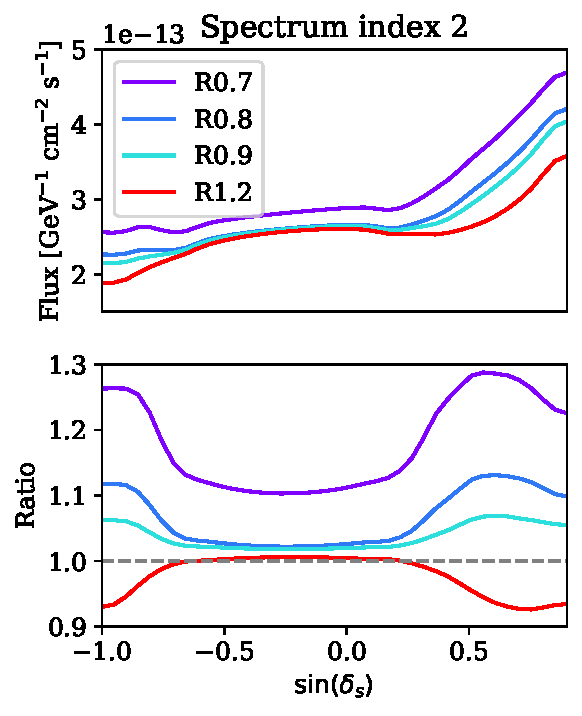
\includegraphics[width=0.45\textwidth]{img/spacing/source_sensitivity_2_hori.pdf}
    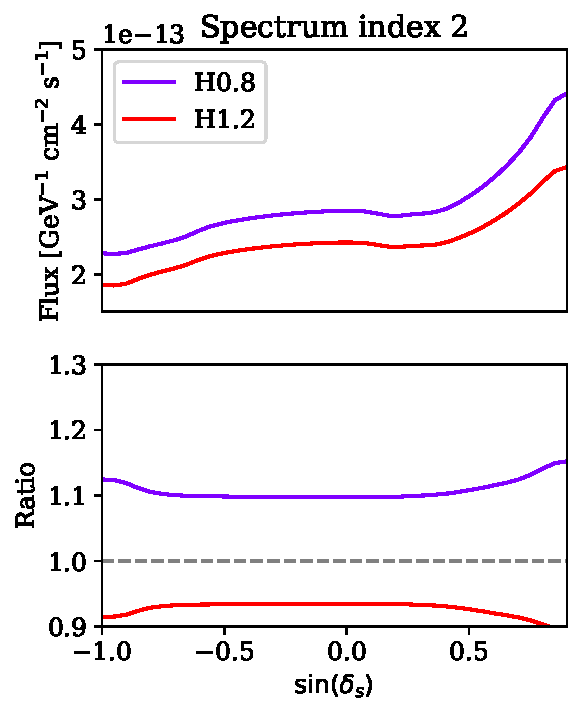
\includegraphics[width=0.45\textwidth]{img/spacing/source_sensitivity_2_vert.pdf}
    \caption{不同的阵列几何间距下,海铃在10年时间内对能谱指数为-2的源的达到$5\sigma$置信度观测所需要的流量。左图表示对水平缩放因子的分析,而右图表示对垂直缩放因子的分析;上图表示绝对角分辨率,而下图表示相对于标准整列配置的角分辨变化。其中红色线表示放大阵列的水平或者垂直间距,而蓝紫色线表示缩小阵列的间距,具体的放大因子参见图注。}
    \label{fig:spacing_source_sensitivity_2}
\end{figure}

\begin{figure}[!htb]%
    \centering
    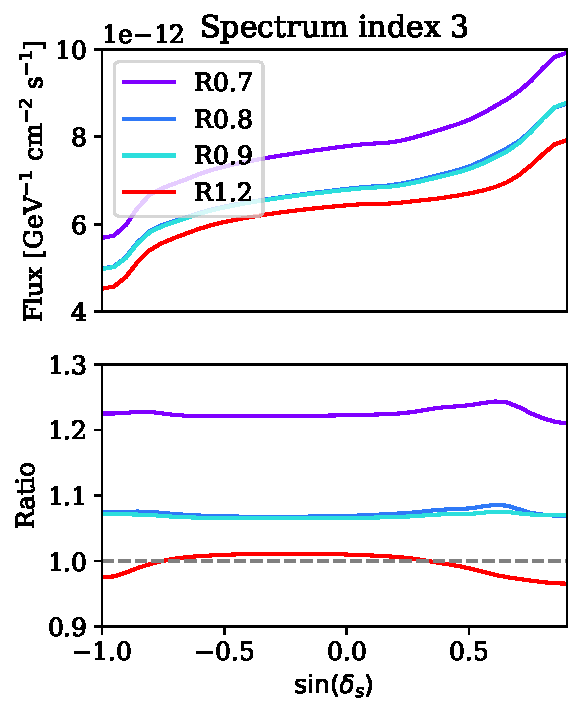
\includegraphics[width=0.45\textwidth]{img/spacing/source_sensitivity_3_hori.pdf}
    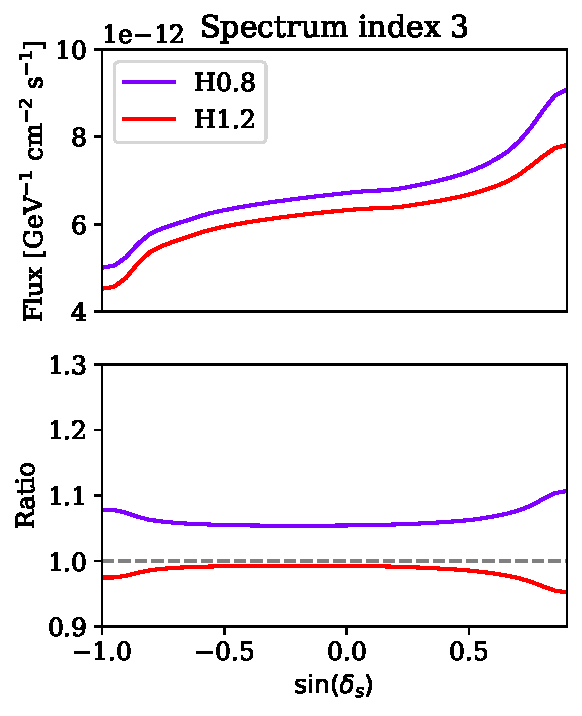
\includegraphics[width=0.45\textwidth]{img/spacing/source_sensitivity_3_vert.pdf}
    \caption{与图\ref{fig:spacing_source_sensitivity_2}类似,但是针对的是能谱指数为-3的源。}
    \label{fig:spacing_source_sensitivity_3}
\end{figure}
